\documentclass[a4paper, 12pt]{article}
\usepackage[utf8]{inputenc}
\usepackage[top=3cm, left=3cm, right=2cm, bottom=2cm]{geometry}
\usepackage{booktabs} % Para inserir bordas na tabela
\usepackage{listings} % Para adicionar trechos de codigo
\usepackage{float} % permite manter a imgem em lugar especifico.
%\usepackage{temp/sbc-template}
\usepackage{graphicx,url}% para inserir imagens e url's
\usepackage{hyperref} %para adicionar hiperligacoes
%\usepackage[brazil]{babel}   
\usepackage[utf8]{inputenc}  


%\sloppy
%\title{Projeto e Analise de Algoritmos\\ Trabalho de Grafos}

%\author{Cristiane\inst{1}, Felipe Rafael \inst{1}, Larissa\inst{1}, Joaquim Armando Dlima Viana\inst{1} }


%\address{Instituto de Ciencias Exatas e Naturais - Universidade Federal do Para (UFPA)\\
	%	Belem -- PA -- Brazil
	%	\email{\{cristiane}@gmail.com, {felipe.rafael@gmail.com}, {larissa}@gamil.com, {jviana}@unilurio.ac.mz}


\begin{document} 
	
	%	\maketitle
	
	
	\section{Problema}
	
	\section{Problema}
	
	\newpage
	
	\section{Problema}
	
	O problema colocado é descrito na literatura como Problema do Carteiro Chines Direcionado. O método que vamos apresentar para solucionar problemas desse tipo foi descrito por Thimbleby (2003) baseado no problema clásssico de transportes apresentado por Beltrami \& Bodin (1972).
	
	Seja um Digrafo $D=(V,A)$ com $V=\{v_1,v_2,v_3,...,v_i\}$ o conjunto de vértices e $A=\{a_1,a_2,a_3,...a_n\}$ o conjunto dos arcos, vamos dar algumas definições:
	
	\textbf{Grau de saída} de $v$ - o número total de vértices saindo de $v$, denotaremos por $d^+(v)$
	 
	\textbf{Grau de entrada} de $v$ - o número total de vértices entrando em $v$, denotaremos por $d^-(v)$
	
	\textbf{Vértice balanceado} - quando o grau de entrada é igual ao grau de saída. Um vértice é balanceado se $\delta(v)=d^(v)-d^-(v)=0$ e desbalanceado nos casos que $\delta \neq 0$.
	
	\textbf{Variáveis de decisão} - denotadas por $x_{i,j}$ a quantidade de arcos a serem acrescentados no caminho $i \rightarrow j$
	
	\textbf{Custo} - denotado por $c_{i,j}$ se refere ao peso do caminho $i\rightarrow j$
	

	Denotaremos por $D^+=\{v| \delta(v) > 0\}$ o conjunto de vértices desbalanceados com excesso de arcos de saída.
	
	Denotaremos por $D^-=\{v| \delta(v) < 0\}$ o conjunto de vértices desbalanceados com excesso de arcos de entrada.
	 
	
	\subsection{Algoritmo}
	
	\begin{enumerate}
		\item Determinar $\delta(v)$ para cada vertice, $D^+$, $D^-$ e $c_{i,j}$.
		
		\item Encontrar a função objetivo $Z$ a ser minimizada. Ela é encontrada resolvendo o seguinte Problema de Programação Linear (PPL):
		
		$$min \sum c_{i,j}x_{i,j}$$
		
		sujeito as seguintes restrições:
		
		$$\sum_{j\in D^+}x_{i,j}=-\delta(i)$$
		$$\sum_{i\in D^-}x_{i,j}=\delta(j)$$
		\begin{flushright}
			$x_{i,j}$ são inteiros positivos.
		\end{flushright}
		
		\item Construir o ciclo euleriano com base no algoritmo de Hierholzer.
		
		
		Na figura \ref{fig:fluxogramaPCCD} mostramos um fluxograma para a solução de problemas deste tipo.
		
		\begin{figure}[H]
			\centering
			\includegraphics[width=14cm]{img/fluxograma para PCCD.png}
			\caption{Fluxograma para o Problema do Carteiro Chinês Direcionado}
			\label{fig:fluxogramaPCCD}
		\end{figure}	
	\end{enumerate}
O Problema do Carteiro Chinês direcionado pode ser facilmente solucionado se todos vértices do dígrafo forem balanceados. Neste trabalho iremos apenas focar em dígrafos que apresentam vértices desbalanceados.
	
	\subsection{Exemplo}
	Seja um dígrafo D orientado e valorado apresentado na figura \ref{fig:grafoG}. Vamos encontrar nele um ciclo euleriano.
	\begin{figure}[H]
		\centering
		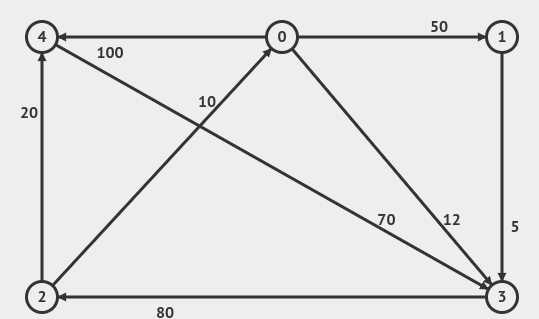
\includegraphics[width=8cm]{img/grafoG.png}
		\caption{Dígrafo D.}
		\label{fig:grafoG}
	\end{figure}
	
	Vamos determinar $\delta(v)$. 
	
	$\delta(0)=2$, $\delta(1)=0$, $\delta(2)=1$, $\delta(3)=-2$ e $\delta(4)=-1$
	
	Os vértices 0, 2, 3 e 4 estão desbalanceados. Apenas o vértice 1 está balanceado. 
	
	Assim podemos criar dois conjuntos $D^-=\{3,4\}$ e $D^+=\{0,2\}$. Juntos formam um subgrafo $D'$, bipartido, contendo os vértices 0, 2, 3 e 4 Como ilustra figura \ref{fig:subgrafoG}
	
	\begin{figure}[H]
		\centering
		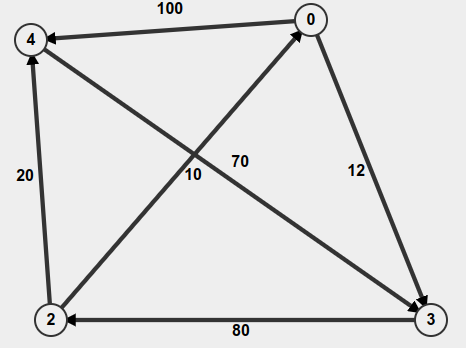
\includegraphics[width=8cm]{img/subgrafoG.png}
		\caption{Subgrafo de G.}
		\label{fig:subgrafoG}
	\end{figure}


 Para determinar os custos $c_{i,j}$ vamos calcular as distâncias mínimas entre os vértices usando o algoritmo de Dijkstra. Em alternativa pode ser também usado o algoritmo de Floyd-Warshall.


\begin{table}[H]
	\centering
	\begin{tabular}{c c r l}
		\toprule[1.5pt]
		\textbf{Origem}  & \textbf{Destino} & \textbf{Distância} & \textbf{Caminho}\\
		\midrule
		0 & 2 & 92 & 0-3-2\\
		0 & 3 & 12 & 0-3\\
		0 & 4 & 100& 0-4\\
		2 & 0 & 10 & 2-0\\ 
		2 & 3 & 22 & 2-0-3\\
		2 & 4 & 20 & 2-4\\
		3 & 0 & 90 & 3-2-0\\
		3 & 2 & 80 & 3-2\\
		3 & 4 & 100& 3-2-4\\
		4 & 0 & 160& 4-3-2-0\\
		4 & 2 & 150& 4-3-2\\
		4 & 3 & 70 & 4-3\\
		\bottomrule[1.5pt]
		
	\end{tabular}
	\caption{Distância mínima entre os vértices usando o Algoritmo de Dijkstra.}
	\label{tab:distancia_minima}
\end{table}

Podemos agora representar os arcos no dígrafo $D'$, de modo que cada arco tenha distância mínima calculada anteriormente. Isso transforma $D'$ em um $K_{12}$. A figura \ref{fig:subgrafoG_Km} ilustra isso:

\begin{figure}[H]
	\centering
	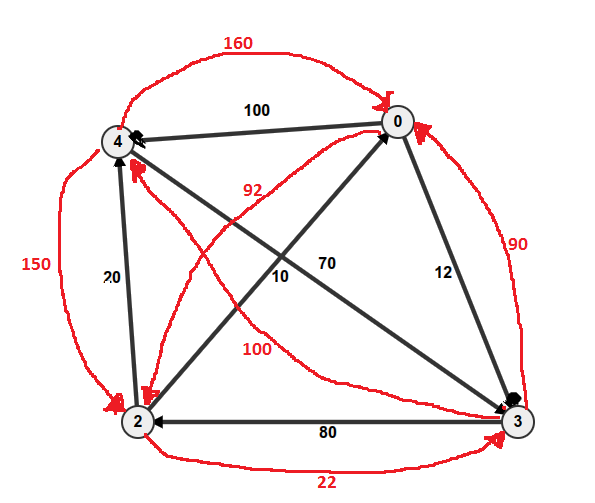
\includegraphics[width=8cm]{img/subgrafoG - Km.png}
	\caption{Subgrafo completo de D com as distâncias mínimas inseridas.}
	\label{fig:subgrafoG_Km}
\end{figure}

O problema agora passa por solucionar quais dos arcos (na cor vermelha) serão mantidos, removidos ou duplicados para que $D'$ tenha um ciclo euleriano com custo mínimo.

Para isso podemos usar o modelo de PPL descrito no passo 2 do algoritmo.

	$min Z$

$Z=92x_{0,2}+12x_{0,3}+100x_{0,4}+10x_{2,0}+22x_{2,3}+20x_{2,4}+90x_{3,0}+80x_{3,2}+100x_{3,4}+160x_{4,0}+150x_{4,2}+70x_{4,3}$

sujeito à:
\begin{itemize}
	\item Restrição para o vértice \textbf{0}: $x_{3,0}+x_{3,2}=2$
	\item Restrição para o vértice \textbf{2}: $x_{4,0}+x_{4,2}=1$
	\item Restrição para o vértice \textbf{3}: $x_{3,0}+x_{4,0}=2$
	\item Restrição para o vértice \textbf{4}: $x_{2,3}+x_{2,4}=1$
\end{itemize}

Os resultados para a execução do modelo de PPL anterior estão descritos na tabela \ref{tab:execucao_PPL}.  Este resultado nos informa que o grafo euleriano será obtido duplicando os arcos no caminho mínimo entre os vértices 3 e 0, entre os vértices 3 e 2 e entre os vértices 4 e 0.


	\begin{table}[H]
		\centering
		\begin{tabular}{l c c c c c c c c c c c c}
			\toprule[1.5pt]
			\textbf{Variável}  & $x_{0,4}$ & $x_{3,0}$ & $x_{0,3}$ & $x_{0,2}$ & $x_{3,4}$ & $x_{4,2}$ & $x_{3,2}$ & $x_{2,3}$ &  $x_{4,0}$ & $x_{2,4}$ & $x_{2,0}$ & $ x_{4,3}$\\
			\midrule
			\textbf{Valor}  & 0 & 1 & 0 & 0 & 0 & 0 & 1 & 0 & 1 & 0 & 0 & 0 \\
			
			\bottomrule[1.5pt]
			
		\end{tabular}
		\caption{Resultado da execução do modelo de PPL.}
		\label{tab:execucao_PPL}
	\end{table}


De acordo com a tabela \ref{tab:distancia_minima} que nos mostra a distancia mínima, no caminho 3 e 0 temos 2 arcos, no caminho 3 e 2 temos 1 arcos e no caminho 4 e 0 temos 3 arcos. Ao todo temos 6 arcos.

A figura mostra o dígrafo após inserção dos novos arcos para formar o ciclo euleriano. 
\begin{figure}[H]
	\centering
	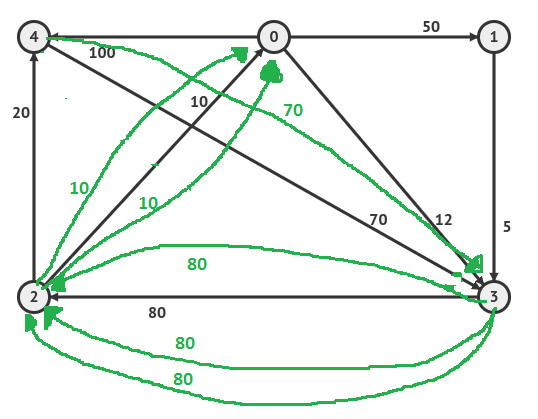
\includegraphics[width=8cm]{img/grafoG - Euleriano.png}
	\caption{Dígrafo D com ciclo euleriano.}
	\label{fig:grafoG - Euleriano}
\end{figure}

O algoritmo de Hierholzer (que é uma variação do algoritmo de Fleury para grafos orientados) pode ser usado para encontrar o ciclo euleriano.
O ciclo euleriano para este exemplo será: 0-3-2-0-4-3-2-0-1-3-2-4-3-2-0. O custo mínimo é obtido somando o peso de todos arcos percorridos, no caso 677.



	\subsection{Complexidade}
	A complexidade do método descrito acima depende do algoritmo usado para solucionar o modelo de PPL. O algoritmo descrito acima quando empregado com o método simplex pode oferecer uma complexidade exponencial dependendo do número de vértices do subgrafo $D$ e do número de restrições. Porém, outros métodos como o método de pontos interiores são mais eficientes e quando empregados torna esse algoritmo eficiente entregando uma complexidade $O(mn^2)$.
	
	\subsection{Código Java}
	Este código está disponível no github \href{https://github.com/feliperasan/Eulerian-Graph}{Clique aqui}
	
	Ou pelo link: https://github.com/feliperasan/Eulerian-Graph
	
	
	

	\newpage
	\section{Referências}
	
	Beltrami, E.J. \& Bodin, L.D.(1972). \textit{Networks and vehicle routing for municipal waste collection}. Report No. UPS 72-18, State University of New York. Stony Brook, NY.
	%\\\\
	%Edmonds, J. and Johnson, EL. \textit{Matching, Euler tours and the Chinese postman}. Mathematical Programming. 5:88–124, 1973.
	\\\\
	Thimbleby, H. (2003). \textit{The directed Chinese Postman Problem}. Softw., Pract. Exper.. 33. 1081-1096. 10.1002/spe.540.
	\\\\
	Verberk, L. (2019). \textit{The Chinese postman problem in undirected and directed graphs}. Eindhoven University of Technology.  
	
\end{document}
